%\documentclass{ctexart}
%\setCJKmonofont{}

\documentclass{article}
\usepackage{tikz}
\usepackage{graphicx}
\usepackage{xeCJK}
%\usepackage{fontspec}
%\setmainfont{Noto Sans CJK SC}

%\usepackage{pgfplots}
%\usepgfplotslibrary{polar}

\begin{document}
\thispagestyle{empty}
\begin{figure}
  \centering
  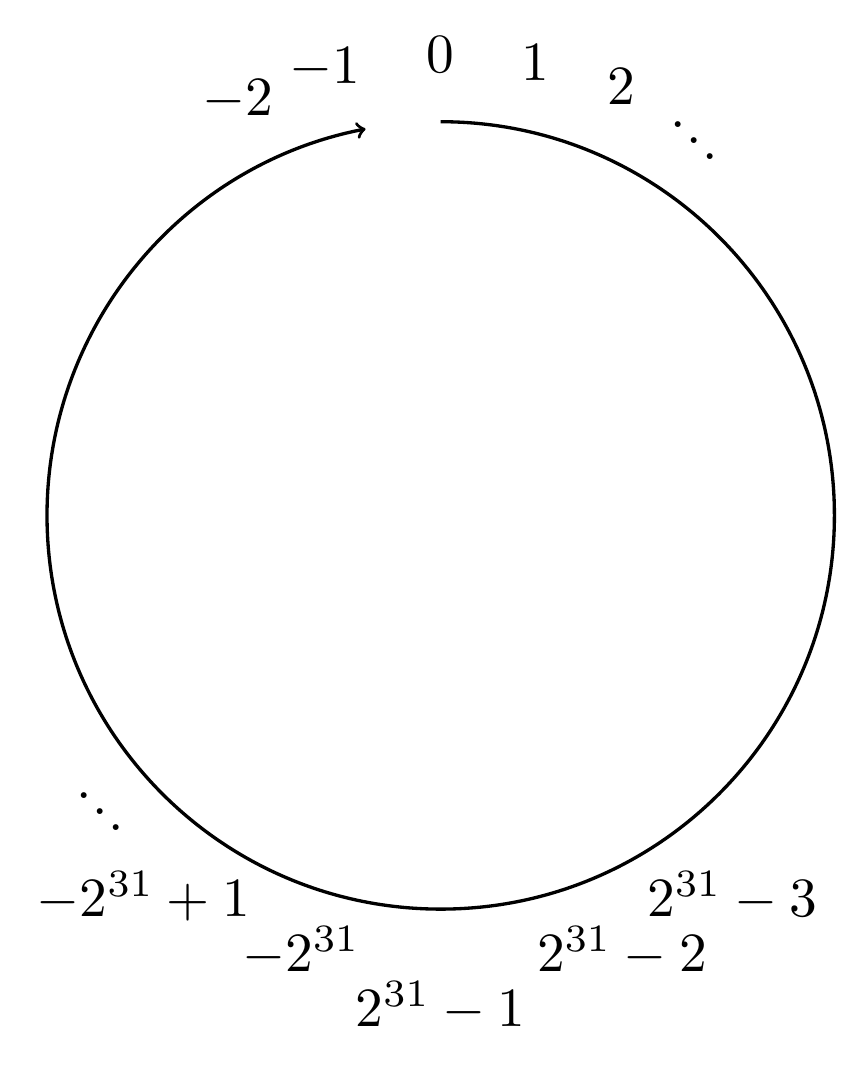
\begin{tikzpicture}
  	%\draw[->] (0,0) circle (5cm);  % -> doesn't work
  	\draw[very thick,->] (0,5) arc (90:-259:5cm);
  
  	% annotate the int
  	%\draw (0,5) node[anchor=south] {$\Large 0$};  % 0 too small
  	%\draw (0,5.5) node[anchor=south] {\scalebox{2}{$\Large 0$}};  % cf. https://tex.stackexchange.com/questions/3703/make-equations-large
  	\node[above]       at (0, 5.5) {\scalebox{2}{$0$}};
  	\node[above right] at (0.9, 5.4) {\scalebox{2}{$1$}};
  	\node[above right] at (2, 5.1) {\scalebox{2}{$2$}};
  	%\node[above right] at (3, 4.7) {\scalebox{2}{.}};
  	\node[above right] at (2.8, 4.8) {\scalebox{2}{.}};
  	%\node[above right] at (3.2, 4.6) {\scalebox{2}{.}};
  	\node[above right] at (3.0, 4.6) {\scalebox{2}{.}};
  	%\node[above right] at (3.4, 4.5) {\scalebox{2}{.}};
  	\node[above right] at (3.2, 4.4) {\scalebox{2}{.}};
  
  	\node[above left] at (-0.9, 5.3) {\scalebox{2}{$-1$}};
  	\node[above left] at (-2, 4.9) {\scalebox{2}{$-2$}};
  	%\begin{polaraxis}
  	%	\draw (4.8,10) -- (5.2,10);
  	%\end{polaraxis}
  
  	%\node[below]       at (0, -5.5) {\scalebox{2}{$127$}};
    \node[below]       at (0, -5.8) {\scalebox{2}{$2^{31}-1$}};
  	%\node[below right] at (0.9, -5.3) {\scalebox{2}{$126$}};
    \node[below right]  at (1.1, -5.1) {\scalebox{2}{$2^{31}-2$}};
  	%\node[below right] at (2.3, -4.8) {\scalebox{2}{$125$}};
    \node[below right] at (2.5, -4.4) {\scalebox{2}{$2^{31}-3$}};
  	%\node[below left] at (-0.9, -5.3) {\scalebox{2}{$-128$}};
    \node[below left] at (-0.9, -5.1) {\scalebox{2}{$-2^{31}$}};
  	%\node[below left] at (-2.3, -4.8) {\scalebox{2}{$-127$}};
    \node[below left] at (-2.3, -4.4) {\scalebox{2}{$-2^{31}+1$}};
  	\node[below left] at (-3.9, -3.8) {\scalebox{2}{.}};
  	\node[below left] at (-4.1, -3.6) {\scalebox{2}{.}};
  	\node[below left] at (-4.3, -3.4) {\scalebox{2}{.}};



  \end{tikzpicture}
	\vspace{1cm}
	\caption{任意兩個整數相加可以看作類似角度上的相加, 角度從$0$算起}
	%\caption{In C, the addition of any two \texttt{signed int} (here for example $8\,$-bit) is nothing more than a compound clockwise rotation along the circle}
  %\label{int_circle}
\end{figure}
\end{document}
